\documentclass[oneside,final,12pt]{extreport}
\usepackage{cmap}
\usepackage{mathtext}
\usepackage[T2A]{fontenc}
\usepackage[utf8]{inputenc}
\usepackage[english,russian]{babel}
\usepackage{vmargin}
\setpapersize{A4}
\setmarginsrb{2.5cm}{2cm}{1.5cm}{2cm}{0pt}{0mm}{0pt}{13mm}
\usepackage{fontspec}
\usepackage{indentfirst}
\usepackage{amssymb,amsmath}
\usepackage[colorlinks,urlcolor=blue]{hyperref}
\usepackage{graphicx}
\sloppy
\flushbottom
\def\baselinestretch{1.2}
\setmainfont{Verdana}
\author{Колосков Андрей Анатольевич}
\begin{document}
\begin{titlepage}
\begin{center}
\Large Московский государственный университет имени М.В. Ломоносова \\[5cm]
\huge Задание 1 \\[0.5cm]
\Large Автоматическое дифференцирование для автокодировщика \\[5cm]
\begin{flushright}
\begin{minipage}{0.8\textwidth}
\normalsize\emph{Факультет:} Вычислительной математики и кибернетики \\
\emph{Кафедра:} Системного программирования \\
\emph{Группа:} 628 \\
\emph{Студент:} Колосков Андрей Анатольевич \\
\emph{Предмет:} Глубинное обучение \\[5cm]
\end{minipage}
\end{flushright}
\large 8 октября 2017
\end{center}
\end{titlepage}
\newpage
\section*{Формулировка задания}
\begin{enumerate}
\item Для модели автокодировщика реализовать процедуру вычисления функции потерь $F(\Theta)$ с помощью прохода вперёд, а также её градиента с помощью прохода назад. Проверить корректность вычислений с помощью разностной аппроксимации;
\item Выписать формулы для прохода назад для оператора $Rp\{·\}$ производной функции-аргумента по заданному направлению $p$, полученные формулы вставить в отчёт. Реализовать процедуру вычисления произведения гессиана функции $F(\Theta)$ на произвольный вектор $p$. Проверить корректность вычислений с помощью разностной аппроксимации;
\item Реализовать процедуру вычисления произведения гаусс-ньютоновской аппроксимации гессиана функции $F(\Theta)$ на произвольный вектор $p$. Для реализованного кода проверить корректность вычислений;
\item Реализовать набор стохастических методов оптимизации: 1) стохастический градиентный спуск (SGD), 2) SGD+momentum, 3) RMSprop и 4) ADAM;
\item Провести исследование с реализованной моделью автокодировщика и методами стохастической оптимизации. Рассмотреть набор данных MNIST1, а также несколько архитектур автокодировщика, в которых на среднем слое находится два нейрона и используется линейная функция потерь. Для различных методов оптимизации построить графики сходимости значения функции потерь на валидационной выборке в зависимости от числа эпох. Прокомментировать использованный способ настройки длины шага и размера мини-батча. Какой из методов оптимизации показывает наилучшие результаты? Визуализировать значения выходов со среднего слоя (там, где два нейрона) для начальных значений параметров автокодировщика и для параметров, найденных в результате оптимизации;
\item Составить отчёт в формате PDF о результатах всех проведённых исследований;
\end{enumerate}
\newpage
\section*{Реализация}
Реализация всех функций прохода вперед и назад для слоя находятся в файле $layers.py$, приложенном к данному отчету.  Реализация функций работы автокодировщика в целом находится в файле $autoencoder.py$. Вычисление функций активации и численного контроля градиентов находятся в файлах $activations.py$ и $check\_grad\_functions.py$ соответственно.

Проверка корректности вычисления прохода вперед---назад с помощью разностной аппроксимации осуществляется в $check\_forward\_backward.py$, запуск:\\


$python3 \ check\_forward\_backward.py$ \\


Получаем результат порядка $1.0e-8$ \ -- \ $1.0e-11$, что сопоставимо с $\varepsilon=\sqrt[]{\varepsilon_{mach}}$, и соответствует заданию.

Формулы для прохода назад оператора $Rp\{·\}$ получены путем применения оператора $Rp\{·\}$ к каждой строчке стандартного алгоритма прохода назад, представленного в задании:\\


$\nabla _{z^L}R_p\{L\} = R_p\{z^L\}$


$\nabla _{u^L}R_p\{L\} = \nabla _{z^L}R_p\{L\} \odot g^\prime(u^L) + \nabla _{z^L}L  \odot g^{\prime\prime}(u^L) \odot R_p\{u^L\}$


$\nabla _{\bar W^L}R_p\{L\} = (\nabla _{u^L}R_p\{L\})(\bar z^{L-1})^T + (\nabla _{u^L}L)(R_p\{\bar z^{L-1}\})^T$


$для l=L-1,L-2,...,1:$


$\nabla _{z^l}R_p\{L\} = (\bar p^{l+1})^T (\nabla _{u^L}L) + (W^{l+1})^T(\nabla _{u^L}R_p\{L\})$


$\nabla _{u^l}R_p\{L\} = \nabla _{z^l}R_p\{L\} \odot g^\prime(u^l) + \nabla _{z^l}L  \odot g^{\prime\prime}(u^l) \odot R_p\{u^l\}$


$\nabla _{\bar W^l}R_p\{L\} = (\nabla _{u^l}R_p\{L\})(\bar z^{l-1})^T + (\nabla _{u^l}L)(R_p\{\bar z^{l-1}\})^T$ \\


Проверка корректности вычисления произведения вычисления произведения гессиана функции $F(\Theta)$ на произвольный вектор $p$ с помощью разностной аппроксимации осуществляется в $check\_rp\_forward\_backward.py$, запуск:\\


$python3 \ check\_rp\_forward\_backward.py$ \\


Получаем результат порядка $1.0e-9$ \ -- \ $1.0e-13$, что сопоставимо с $\varepsilon=\sqrt[]{\varepsilon_{mach}}$, и соответствует заданию.


Проверка корректности вычисления произведения гаусс-ньютоновской аппроксимации гессиана функции $F(\Theta)$ на произвольный вектор $p$ с помощью разностной аппроксимации осуществляется в $check\_gauss\_newton.py$, запуск:\\


$python3 \ check\_gauss\_newton.py$ \\


Получаем результат порядка $1.0e-8$ \ -- \ $1.0e-10$, что сопоставимо с $\varepsilon=\sqrt[]{\varepsilon_{mach}}$, и соответствует заданию.


Стохастический градиентный спуск (SGD), SGD+momentum, RMSprop и ADAM реализованы в файле $autoencoder.py$. Их использование в файле $use\_autoencoder.py$, запуск:



\begin{verbatim}
python3 use_autoencoder.py -p <path to MNIST folder> 
         -t <type of gradient function> -tr <train data size> 
         -ts <test data size> -e <number of epochs> -ms <minibatch size> 
         -mm <momentum> -d <print to display>
\end{verbatim}


В результате тестирования на наборе данных MNIST нескольких моделей автокодировщика со средним слоем 2 нейрона и линейной функцией потерь, наилучшую сходимость удалось достигнуть при небольшом числе слоев и резких изменениях в количестве нейронов между слоями: 784, 250, 50, 2, 50, 250, 784.


Длина шага определяется согласно рекомендациям: \href{http://www.machinelearning.ru/wiki/index.php?title=Практикум_на_ЭВМ_(317)/2012-2013/Autoencoder}{практикум на ЭВМ (317)/2012-2013/Autoencoder}. Зависит от номера эпохи: \\


$s_0 = 1.0$
$s_k = \frac{s_0}{k^{\frac{1}{4}}}$ \\


Это представляется логичным, так как с ростом количества эпох, величина функции потерь снижается и градиентный спуск должен осуществляться более мелкими шагами. Размер мини-батча выбирал исходя из того, чтобы туда гарантированно попадала каждая цифра несколько раз, это должно уменьшить вероятность переобучения. Соответственно, он должен быть не менее 100, но не более 1000, так как в противном случае происходит незначительное замедление вычислительного процесса из-за операций с большими матрицами.


Кроме того, немного модифицировал стандартную батч нормализацию. Дело в том, что если преобразовывать входные данные к единичной дисперсии, то значения некоторых точек будут больше 1.0, но так как в сети используется сигмоид, то на выходе все значения будут не больше 1.0. Это увеличит размер ошибки. Поэтому все значения входной выборки делю на максимальное значение плюс 1.0. В данном примере это 256. Таким образом гарантированно получаю значения меньше 1.0 и относительно нормальную сходимость.


На рисунке \,\ref{loss_figure} представлен график сходимости значения линейной функции потерь (вертикальная ось) на валидационной выборке в зависимости от числа эпох (горизонтальная ось) для стохастического градиентного спуска - sgd. Размер тренировочной выборки 1000, тестовой 100, размер мини-батча 100.


\begin{figure}[th]
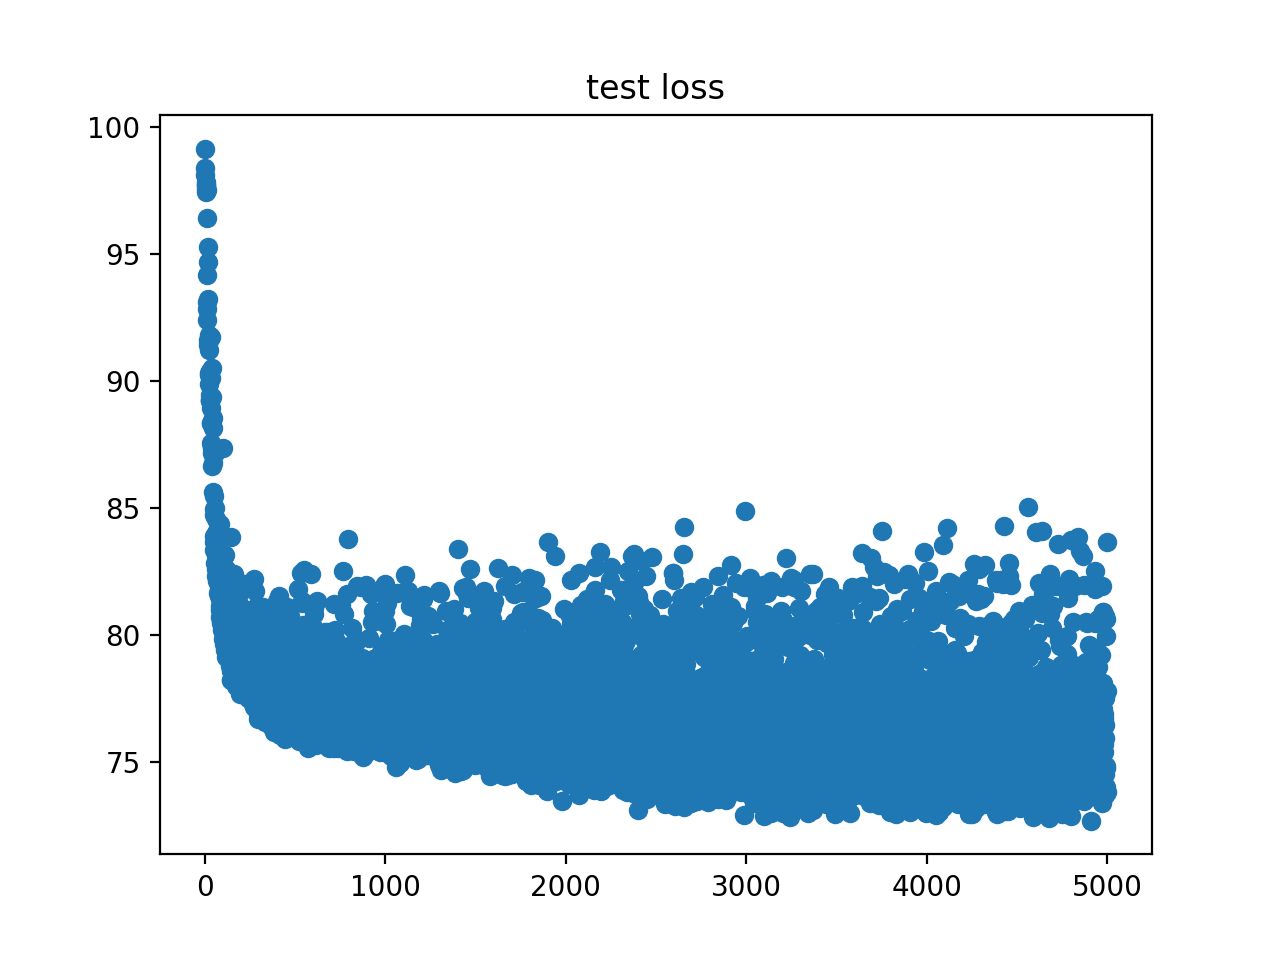
\includegraphics[width=1.0\textwidth]{Figure_2}
\caption{Функция потерь для SGD}
\label{loss_figure}
\end{figure}


Вначале происходит резкое снижение величины функции потерь, а затем ее постепенное плавное снижение, но при этом растет дисперсия. Оптимальное значение функции потерь достигается примерно на 3000 эпохе. Достаточно высокие значения обусловлены тем, что в центральном слое расположено всего 2 нейрона. Эксперименты с большим числом нейронов показывали значительное улучшение данного показателя.


При этом первоначальная картинка в большинстве случаев восстанавливается до приемлемого качества. На рисунках \,\ref{image1} и \,\ref{image2} с левой стороны показаны примеры исходной картинки из тестовой выборки, а справа этой же картинки после прохода через автокодировщик, обученный на 3000 эпохах. Конечно попадаются и плохие варианты, когда происходит сильное искажение, но их значительно меньше. 


\begin{figure}[th]
\begin{minipage}[h]{0.49\linewidth}
\center{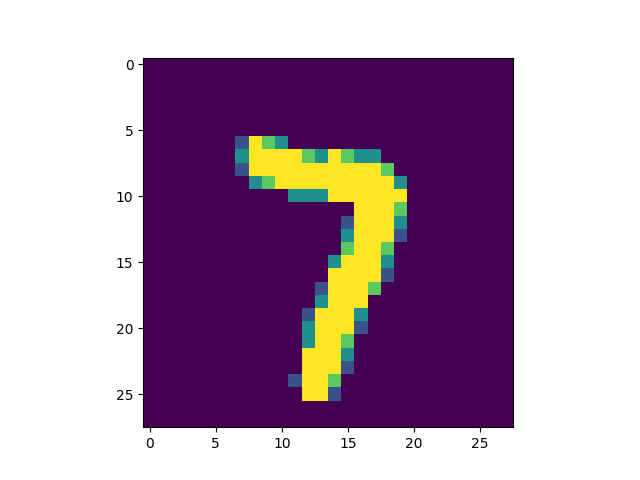
\includegraphics[width=1.0\linewidth]{input1}}
\end{minipage}
\hfill
\begin{minipage}[h]{0.49\linewidth}
\center{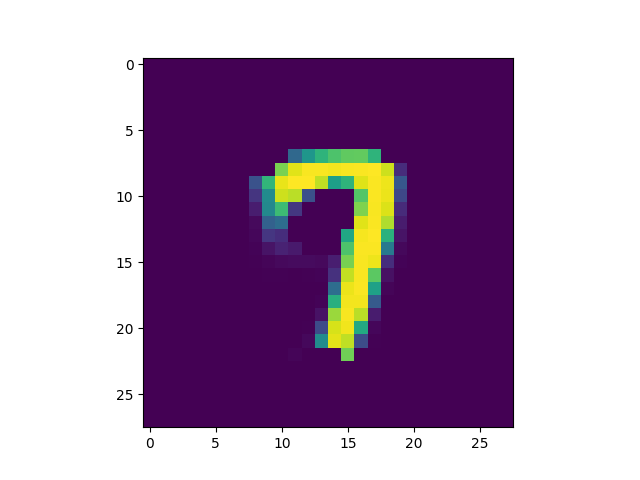
\includegraphics[width=1.0\linewidth]{output1}}
\end{minipage}
\caption{Пример картинки до и после преобразования}
\label{image1}
\end{figure}


\begin{figure}[th]
\begin{minipage}[h]{0.49\linewidth}
\center{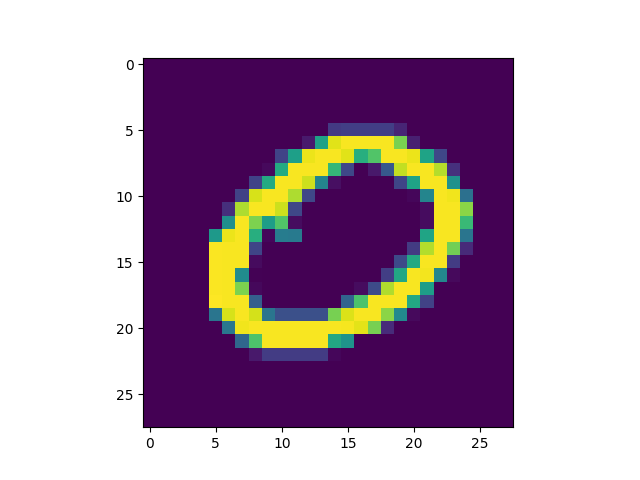
\includegraphics[width=1.0\linewidth]{input4}}
\end{minipage}
\hfill
\begin{minipage}[h]{0.49\linewidth}
\center{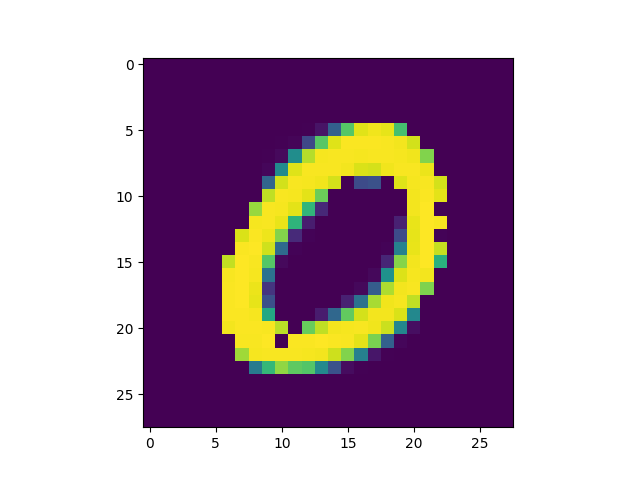
\includegraphics[width=1.0\linewidth]{output4}}
\end{minipage}
\caption{Пример картинки до и после преобразования}
\label{image2}
\end{figure}


На рисунке \,\ref{loss_figure2} представлен аналогичный предыдущему график сходимости значения линейной функции потерь для sgd + momentum. Здесь наблюдается некоторое улучшение относительно простого sgd, немного снизилась величина функции потерь, и уменьшилась дисперсия.


\begin{figure}[th]
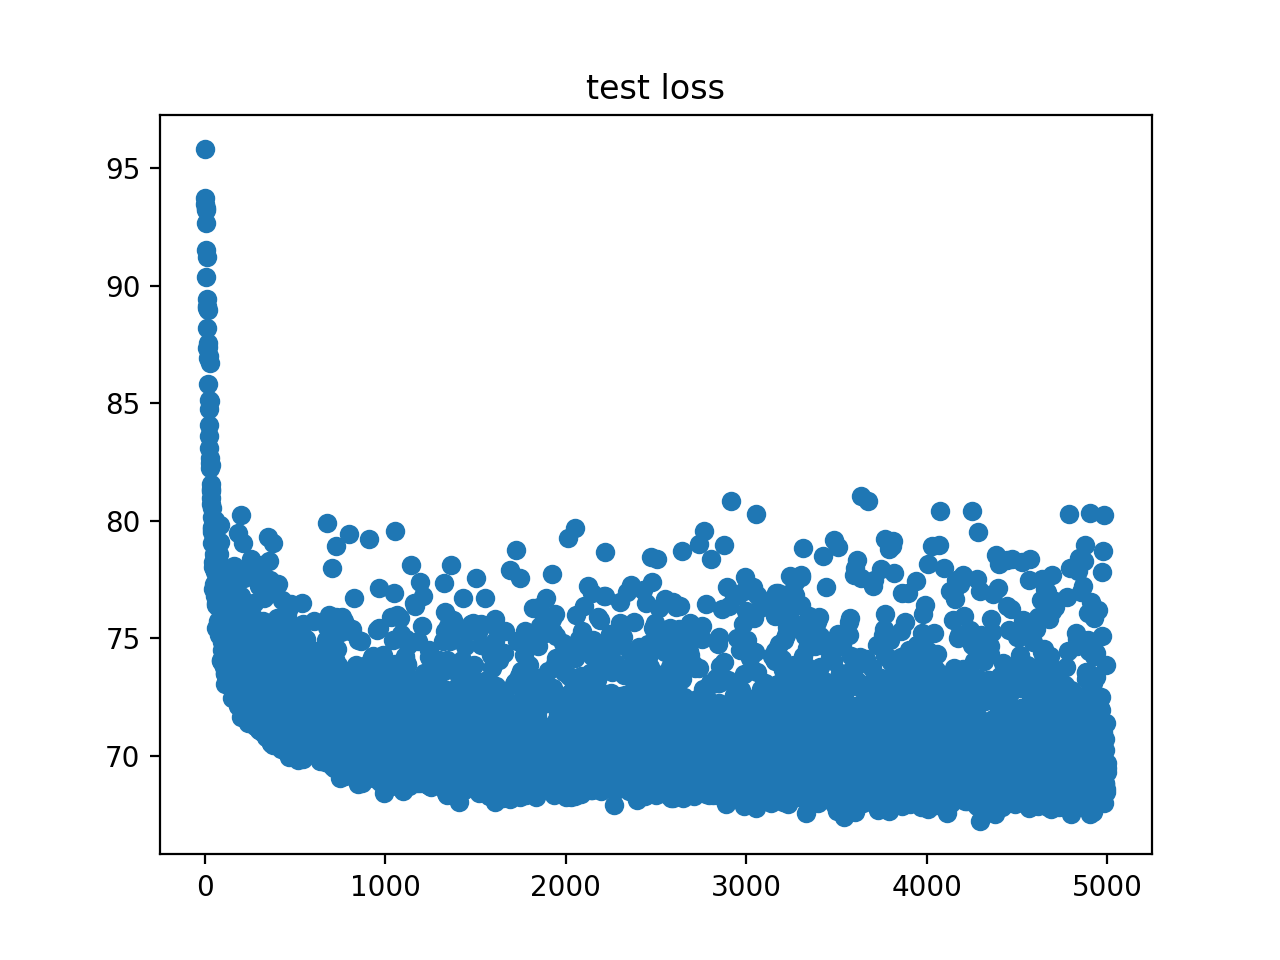
\includegraphics[width=1.0\textwidth]{Figure_3}
\caption{Функция потерь для SGD+momentum}
\label{loss_figure2}
\end{figure}


На рисунке \,\ref{loss_figure3} представлен аналогичный предыдущему график сходимости значения линейной функции потерь для RMSprop. Здесь наблюдается еще большее улучшение относительно sgd и sgd+momentum, снизилась величина функции потерь, и значительно уменьшилась дисперсия.


\begin{figure}[th]
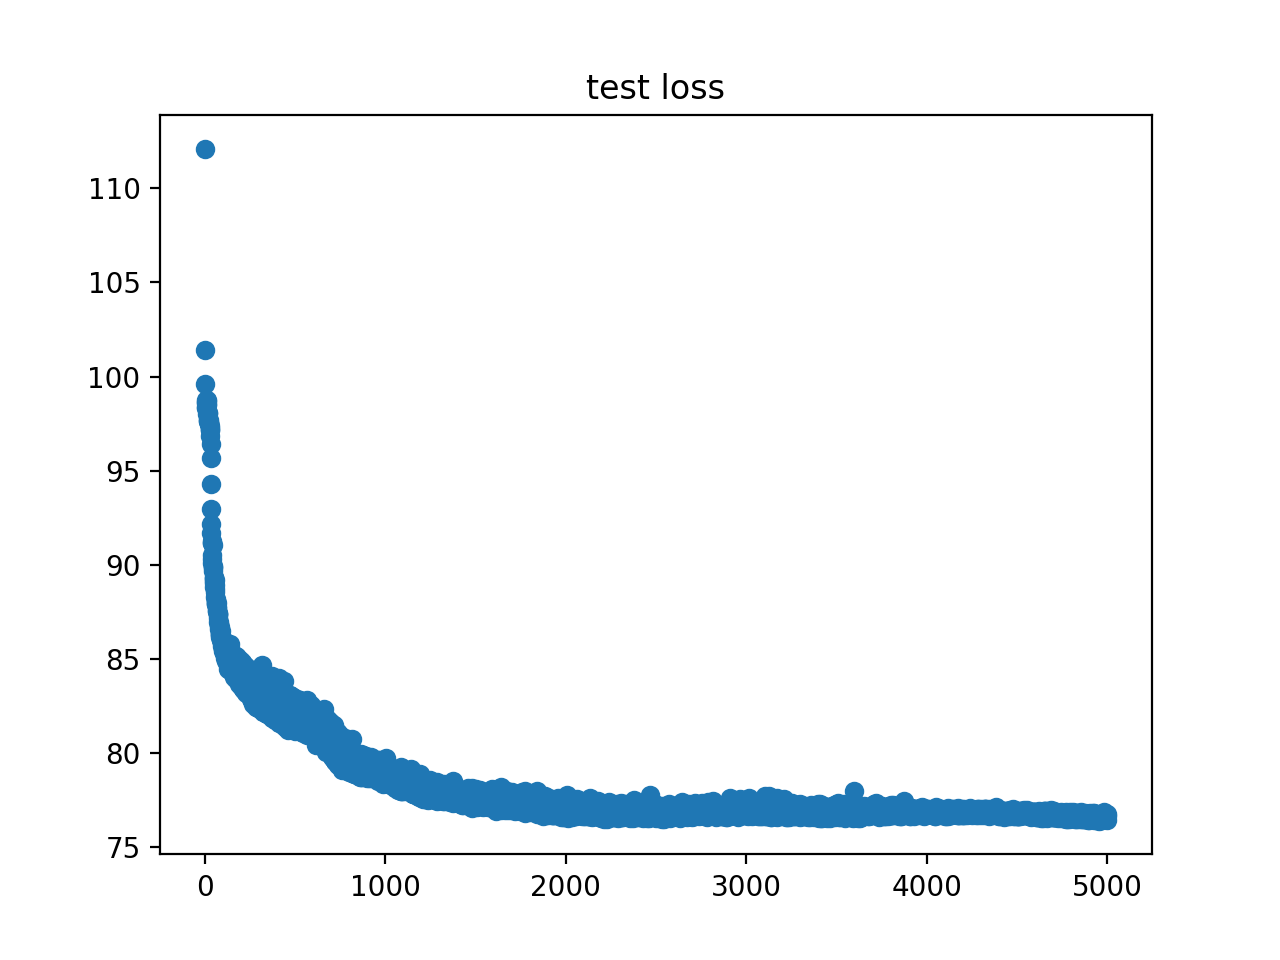
\includegraphics[width=1.0\textwidth]{Figure_6}
\caption{Функция потерь для RMSprop}
\label{loss_figure3}
\end{figure}


На рисунке \,\ref{loss_figure4} представлен аналогичный предыдущем график сходимости значения линейной функции потерь для ADAM. Здесь улучшений не наблюдается, все примерно на уровне предыдущего метода.


\begin{figure}[th]
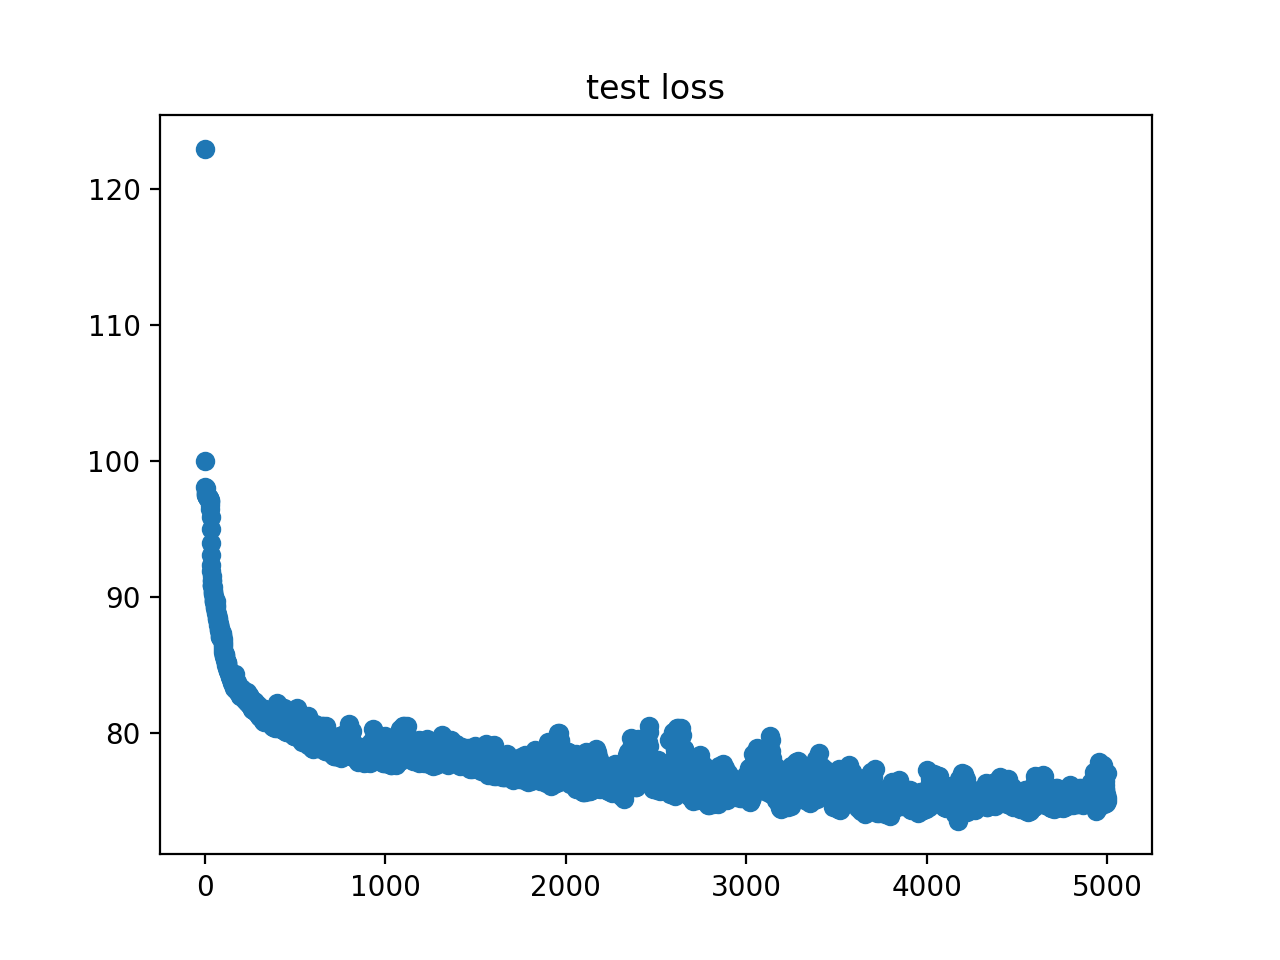
\includegraphics[width=1.0\textwidth]{Figure_7}
\caption{Функция потерь для ADAM}
\label{loss_figure4}
\end{figure}


На рисунке \,\ref{loss_figure5} представлена визуализация среднего слоя для начальных значений автокодировщика, а на рисунке \,\ref{loss_figure6} после оптимизации.
\begin{figure}[th]
\begin{picture}(500,500)(0,0)
\put(50,250){\vector(1,0){100}}
\put(50,150){\vector(1,0){100}}
\put(50,50){\vector(1,0){100}}
\put(170,250){\circle{100}}
\put(170,150){\circle{100}}
\put(170,50){\circle*{5}}
\put(190,250){\vector(1,0){100}}
\put(190,150){\vector(1,1){100}}
\put(190,50){\vector(1,2){100}}
\put(310,250){\circle{100}}
\put(310,150){\circle{100}}
\put(80,260){$0.2433$}
\put(80,160){$-0.0161$}
\put(80,60){$0.1862$}
\put(150,280){$0.1355$}
\put(150,180){$0.2684$}
\put(160,60){$1.0$}
\put(210,260){$0.033$}
\put(200,210){$-0.0043$}
\put(205,150){$0.1862$}
\put(290,280){$0.2149$}
\put(300,50){$...$}
\end{picture}
\caption{Визуализация среднего слоя для начальных значений}
\label{loss_figure5}
\end{figure}


\begin{figure}[th]
\begin{picture}(500,500)(0,0)
\put(50,250){\vector(1,0){100}}
\put(50,150){\vector(1,0){100}}
\put(50,50){\vector(1,0){100}}
\put(170,250){\circle{100}}
\put(170,150){\circle{100}}
\put(170,50){\circle*{5}}
\put(190,250){\vector(1,0){100}}
\put(190,150){\vector(1,1){100}}
\put(190,50){\vector(1,2){100}}
\put(310,250){\circle{100}}
\put(310,150){\circle{100}}
\put(80,260){$3.1177$}
\put(80,160){$1.5588$}
\put(80,60){$0.3570$}
\put(150,280){$0.6207$}
\put(150,180){$0.3015$}
\put(160,60){$1.0$}
\put(210,260){$1.9352$}
\put(200,210){$0.4700$}
\put(205,150){$0.3570$}
\put(290,280){$2.7622$}
\put(300,50){$...$}
\end{picture}
\caption{Визуализация среднего слоя после оптимизации}
\label{loss_figure6}
\end{figure}


По итогам данной работы можно сделать вывод, что модель автокодировщика со средним слоем в 2 нейрона достигает приемлемого качества, но для улучшения показателей все--таки желательно большее количество нейронов.
\end{document}
